\documentclass[a4paper,12pt]{article}

\usepackage[utf8]{inputenc}
\usepackage{graphicx}
\usepackage{xcolor}

%\usepackage[defaultmono]{droidmono}
\usepackage{wrapfig} % Side figure
\usepackage{caption}
\usepackage{subcaption}

\usepackage{amsmath,amssymb,amsthm,textcomp}
\usepackage{fixmath} % Bold text in mathmode
\usepackage{mleftright} % For drawing lines in matrix
\usepackage{enumerate}
\usepackage{multicol}
\usepackage{tikz}

\usepackage{geometry}
\geometry{total={210mm,297mm},
left=25mm,right=25mm,%
bindingoffset=0mm, top=20mm,bottom=20mm}


\linespread{1.3}

\newcommand{\linia}{\rule{\linewidth}{0.5pt}}

% custom theorems if needed
% my own titles
\makeatletter
\renewcommand{\maketitle} {
\begin{center}
\vspace{2ex}
{\huge \textsc{\@title}}
\vspace{1ex}
\\
\linia\\
\@author \hfill \@date
\vspace{4ex}
\end{center}
}
\makeatother
%%%

% custom footers and headers
\usepackage{fancyhdr}
\pagestyle{fancy}
\lhead{}
\chead{}
\rhead{}
\lfoot{FMCS:CS - Part 3}
\cfoot{Page \thepage}
\rfoot{15M54097}
\renewcommand{\headrulewidth}{0pt}
\renewcommand{\footrulewidth}{0pt}
%

% code listing settings
\usepackage{listings}
%%%----------%%%----------%%%----------%%%----------%%%

\newcommand*{\quoteTitle}[1]{{#1}\ignorespaces}%
\newenvironment{Quote}[1]{
    \medskip\par\noindent\quoteTitle{#1}
    \par\noindent
    \begin{quote}
    }{
    \end{quote}
    \par\noindent\ignorespacesafterend
}

\newtheorem{theorem}{Theorem}

\begin{document}
\bibliographystyle{acm}
\title{Fundamentals of MCS: CS - Part 3}

\author{NGUYEN T. Hoang - SID: 15M54097}

\date{Fall 2015, W832 Mon. Period 7-8 \\ \hfill Due date: 2015/02/15}

\maketitle

\vspace{10em}
\section*{Problem}
\noindent
\paragraph{Q2} Summarize and discuss the paper: \\
\hspace{3em} K. Goto, R. Geijin. \emph{Anatomy of high-performance Matrix Multiplication}, ACM TOMS 2008, 25 pages.
\pagebreak




\section{Introduction}

\noindent
In this assignment, I will summarize and discuss the paper named: ``\emph{Anatomy of high-performance Matrix Multiplication}'' by Kazushige Goto and Robert van de Geijn of University of Texas at Austin. This paper, which was published in ACM Transactions on Mathematical Software, Volume 34 Issue 3, May 2008, addresses the \emph{marco} issues about utilizing the high performance \emph{inner-kernel} to implement ``near optimal'' performance of matrix multiplication. Using the layered approach suggested and analyzed by \cite{gunnels2001} and \cite{gunnels2005}, the authors analyzed the computational and memory operation time cost for each matrix multiplication scheme. Based on their high level analysis and observation, they argue that there is a superior inner-kernel to use for matrix multiplication under some practical assumptions and also present some empirical configurations and performance result on different CPU architectures.

\emph{About the main author: } This paper's main author is Kazushige Goto \cite{gototx}. He is a research associate at the Texas Advanced Computing Center at The University of Texas at Austin. Being specialized in super-computing, Goto was addressed as a ``world-class resource'' by Dr. Mark Seager of Lawrence Livermore National Laboratory. As mentioned in the University of Texas at Austin's website, by the year 2006, four of the 11 fastest supercomputers in the world use Goto's code to benchmark their performance. His talent and specialty is shown in his series of publishing about high-performance computing, the one I will summarize here is one vivid example.

My summary of the paper \cite{goto2008} has the following structure: \textbf{Section 2} provides terms and the contribution of the paper. \textbf{Section 3} presents structure and main idea of the paper. \textbf{Section 4} discusses the paper's results and significant. \textbf{Section 5} provides my conclusion about the paper.

\section{Terms and contribution}

\noindent
Matrix multiplication is one of the most used operation in computing science since the matrix representation is useful for modeling real world problems. In a computer's world, the memory is used to store matrix (a 2-D abstract entity) is a 1-dimensional array. Therefore, the designers have to decide whether to store matrix as column-major or row-major order. In this paper I am summarizing here, the authors assumes all matrix representation is column-major order.

\subsection{Terms}
\paragraph{Layered approach} is to decompose matrix multiplication into nested iterations. Each iteration loop is considered one layer. Figure~\ref{fig:layered} represents my annotation of Figure 4 in the original paper \cite{goto2008}.

\begin{figure}[h]
    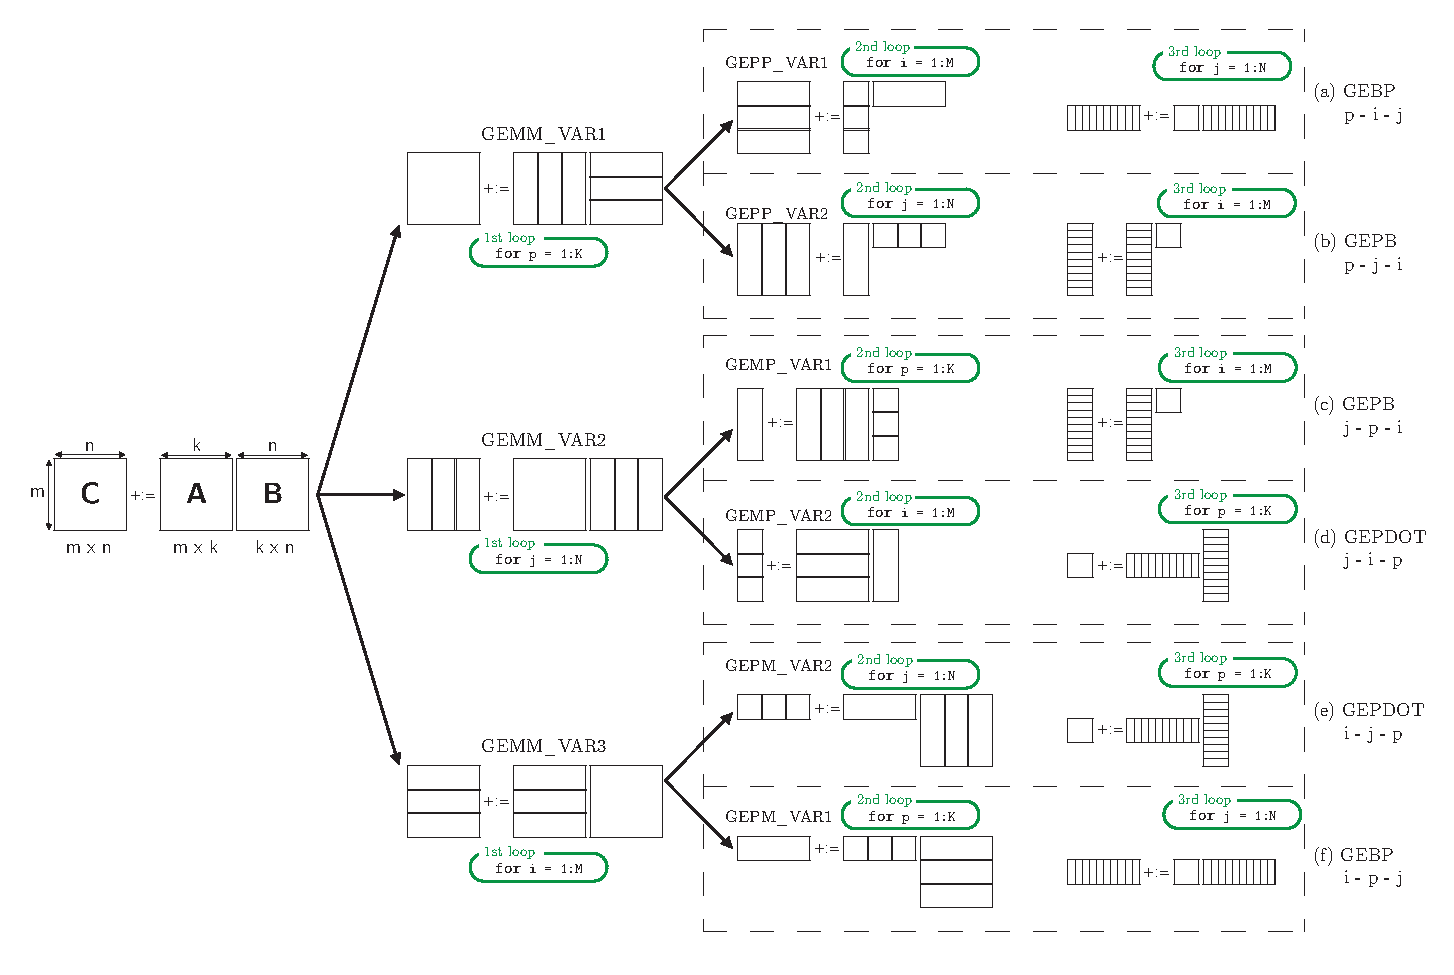
\includegraphics[width=\textwidth]{fmcs_a3_layered}
    \caption{\emph{Layered approach to implementing GEMM annotated.} \cite{goto2008}}
    \label{fig:layered}
\end{figure}

\paragraph{$\mathbold{C:= \tilde{A}B + C}$} is a general matrix multiplication in computing. $\tilde{A}$ is the notation of matrix $A$, but stored contiguously in memory for faster access.
\vspace{-1em}
\paragraph{DGEMM} stands for Double-precision General Matrix-Matrix multiplication.
\vspace{-1em}
\paragraph{GotoBLAS} (now: GotoBLAS2) is Basic Linear Algebra Subprograms written by Goto.
\vspace{-1em}
\paragraph{level-3 BLAS} is a class of BLAS routines that deals with general matrix-matrix multiplication including complex matrix.
\vspace{-1em}
\paragraph{inner-kernel} is the term authors of this paper use to indicate the fundamental computational block used to implement general matrix multiplication.
\vspace{-1em}
\paragraph{LAPACK} is Linear Algebra Package, written in Fortran 90.
\vspace{-1em}
\paragraph{Memory hierarchy} is a high-level view of memory operations in the computer. As in this paper, the refined memory model is demonstrated in Figure~\ref{fig:mem} (a).
\begin{figure}[h]
    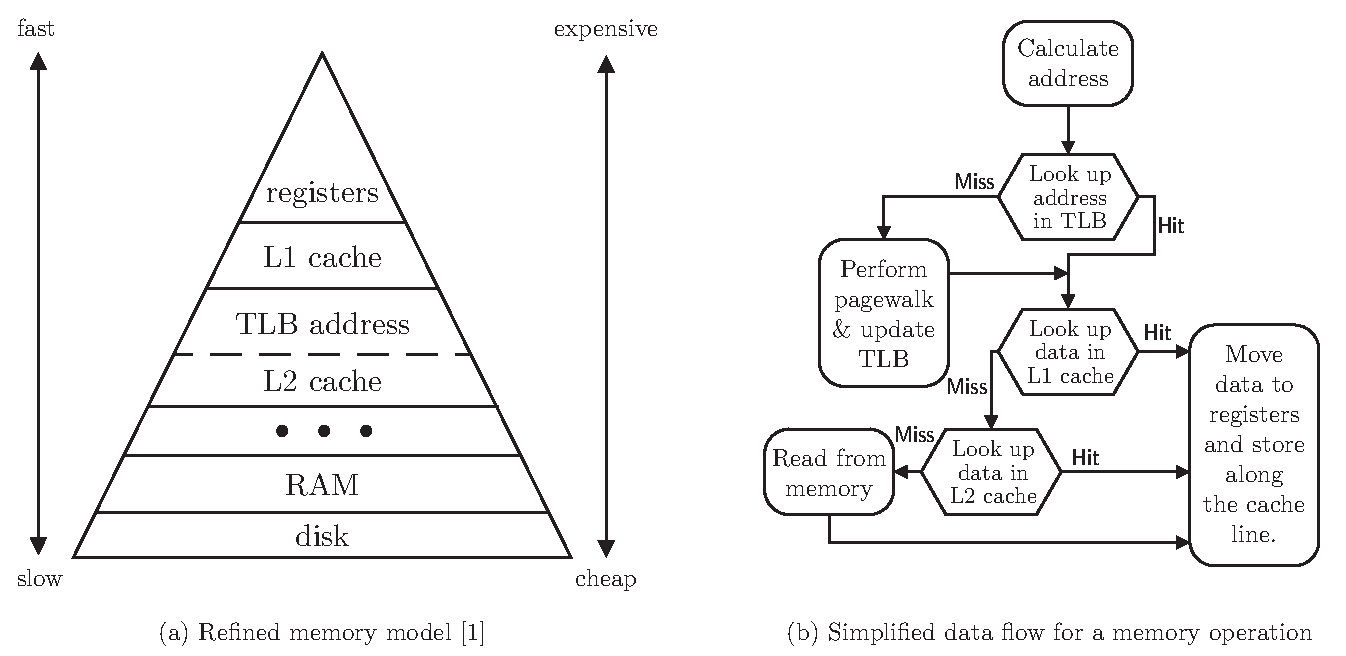
\includegraphics[width=\textwidth]{fmcs_a3_mem}
    \caption{\emph{Refined memory model and simplified memory operation.}}
    \label{fig:mem}
\end{figure}
\paragraph{TLB} is Translation Look-aside Buffer. This hardware feature speeds up Virtual Memory operation of the computer. It acts as a buffer for the page table, in order to increase the speed of translating virtual memory addresses to physical memory addresses.


\subsection{Contribution}
\noindent
This paper has given a systematic analysis of high-level issues that affect the design of high-performance matrix multiplication. By analysis details of each computational scheme, the authors suggested the design parameters and constrains that is arguably achieve ``near optimal'' performance. Besides the analysis and implementation details, the authors also proved the correctness of their design using empirical data on different computing hardware (CPU). The work in this paper can be used as a reference as well as a benchmark method for high performance computation.





\section{Approach and method}

\subsection{Background}
There is 2 main problems and 3 key observations that motivated the work of the authors:
\begin{enumerate}
    \setlength{\parskip}{0cm}
    \setlength{\itemsep}{0cm}
    \item Problem with current analysis:
        \begin{itemize}
            \setlength{\parskip}{0cm}
            \setlength{\itemsep}{0cm}
            \item Assumes that $\tilde{A}$ can fit entirely in cache Level-1 (L1).
            \item Ignore the existence of the Translation Lookaside Buffer (TLB).
        \end{itemize}
    \item Observation:
        \begin{itemize}
            \setlength{\parskip}{0cm}
            \setlength{\itemsep}{0cm}
            \item The rate of moving data from cache Level-2 (L2) to register is roughly equals the floating operation rate of the CPU (at the time this paper was written).
            \item The TLB size is the limit factor of $\tilde{A}$.
            \item There is 6 inner-kernels that are used as building elements for matrix multiplication. The authors argue that under some assumption and design decision, one of those 6 will be a superior choice compare to others.
        \end{itemize}
\end{enumerate}

From these key observations, the authors proposed a detailed analysis using the refined memory model in Figure~ref{fig:mem} (a). By considering the constrains introduced by L1 size and TLB size, they decided to store $\tilde{A}$ in L2 and presented the constrains for block sizes depends on the size of TLB available. There are 5 main assumptions made by the authors in this paper:
\begin{enumerate}
    \setlength{\parskip}{0cm}
    \setlength{\itemsep}{0cm}
    \item The dimensions $m_c, k_c$ (size of matrices in an inner-kernel) are small enough so that $A$ and $n_r$ columns from each of $B$ and $C$ ($B_j$ and $C_j$, respectively) together fit in the cache.
    \item If $A, C_j,$ and $B_j$ are in the cache then $C_j := AB_j + C_j$ can be computed at the peak rate of the CPU.
    \item If A is in the cache it remains there until no longer needed.
    \item The dimensions $m_c, k_c$ are small enough so that $A, n_r$ columns from $B$ $(B_j)$ and $n_r$ column from $C$ $(C_j)$ are simultaneously addressable by the TLB so that during the computation there is no TLB misses occur.
    \item If $A$ is addressed by the TLB, it remains so until no longer needed.
\end{enumerate}

In order to address the problem of matrix-matrix multiplication, the authors break a matrix down to smaller submatrices, or blocks as follow:
$$ X = (X_0 | X_1 | \ldots | X_{N-1}) =
\renewcommand\arraystretch{1.3}
\mleft(
\begin{array}{c}
    \check{X}_0 \\
    \hline
    \check{X}_1 \\
    \hline
    \ldots \\
    \hline
    \check{X}_{N-1} \\
\end{array}
\mright)
$$

 Figure~\ref{fig:mat} gives better visualization of the author intention. The last partition (block column $X_{N-1}$ or block row $\check{X}_{N-1}$) might not have full element.

 \begin{wrapfigure}{r}{0.4\textwidth}
    \vspace{-1em}
    \centering
        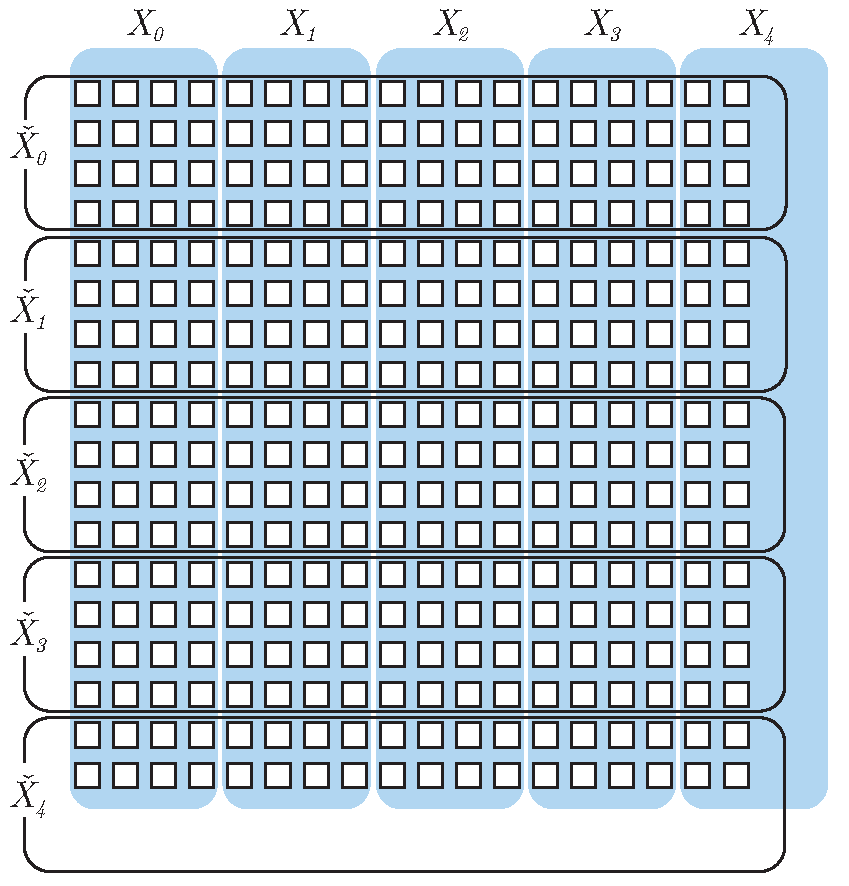
\includegraphics[width=0.38\textwidth]{fmcs_a3_block}
    \vspace{-1em}
    \caption{\emph{Illustration of matrix $X$.}}
    \label{fig:mat}
    \vspace{-2em}
\end{wrapfigure}

As illustrated in Figure~\ref{fig:layered}, any matrix-matrix multiplication can be broken down to smaller (tiny) sub-matrix multiplication. There are two factor in the computing time: The floating point computation time itself and the moving cost to copy data to registers in CPU and write it back to memory. In order to achieve the best performance, the cost of moving data to faster memory should be amortized among the floating point operations. To analyze this matter, the authors of this paper introduces a maximization problem with constrains, the algorithm is illustrated in Figure~\ref{fig:GEBP}:
\[
\begin{cases}
    \mbox{Maximize } \frac{\mbox{computation}}{\mbox{data movement}} = \displaystyle \frac{2m_ck_c}{2m_c+k_c} \\
    m_ck_c \mbox{ floating point numbers fill most of the cache} \\
    \mbox{Assumptions (1) - (3) are met.}
\end{cases}
\]

 \begin{wrapfigure}{rh}{0.5\textwidth}
    \vspace{-1em}
    \centering
        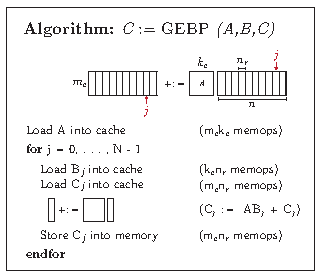
\includegraphics[width=0.48\textwidth]{fmcs_a3_GEBP}
    \vspace{-1em}
    \caption{\emph{Basic implementation of GEBP}.}
    \label{fig:GEBP}
    \vspace{-3em}
\end{wrapfigure}

Base on this analysis, we can see that if $m_c = k_c \approx n/100$, then memops takes only about 10\% overhead to the computation even if it is 10 times slower than flops.

\subsection{Analysis in detail}
In the case of GEBP in Figure~\ref{fig:GEBP}, we need to keep matrix $A$ in the cache during the operation because the iteration keeps accessing data from $A$. On the other hand, the size of L1 is too small to hold all $C_j$, $B_j$, and $A$. Therefore, the author decided to store $A$ in L2 and store others in L1. Denote the computational rate and registers data loading rate as $R_{comp}$ and $R_{load}$. To make moving $A$ to register worth the time, it is necessary to make sure the computing time is larger than the data load time. In this analysis, the authors made one extra assumption that there is ``sufficient bandwidth'' between L1 cache and the register so that moving data from there to register have negligible cost.
\begin{equation*}
    \begin{aligned}
        \centering
        \mbox{computing time } & \ge \mbox{ loading time} \\
        \frac{2c_ck_cn_r}{R_{com}} & \ge \frac{m_ck_c}{R_{load}} \\
        n_r & \ge \frac{R_{com}}{2R_{load}}
    \end{aligned}
\end{equation*}

Another consideration is TLB size. This buffer is a hardware accelerator for the paging procedure of the CPU. As depicted in Figure~\ref{fig:mem} (b), to request data, the CPU will first translate the virtual address to physical address using the page table with its buffer - the TLB. Unlike cache miss, where the system can handle a few while still maintain its overall speed, a TLB miss will cause a page walk and TLB rebuild, which will cost the system a lot of time. Therefore, according to the authors, we have to make sure there is no TLB miss in the entire GEBP operation (assumption 4-5).

The last problem we need to consider is \emph{packing}. Since we break down a large matrix into smaller submatrices, all submatrices will not be in continuous memory array. This segmentation problem will cause memory access more complicated and also it will require more TLB entry to address matrix $A$. To solve this problem, this paper's approach is to pack matrix $A$ into a contiguous form $\tilde{A}$ in memory for faster access (and also do the same for $B$ and $C$ if they are needed in multiple iteration). By saying ``\emph{pack} matrix $A$'' into $\tilde{A}$, it means that the CPU will copy a block of $A$ into a physically contiguous work buffer, $\tilde{A}$. The result is that $\tilde{A}$ is stored in the L2 cache and requires a minimum number of TLB entries. \cite{goto2008}.

To decide the size of matrix $A$ (or packed from $\tilde{A}$) for implementation, the authors considered two limiting factors. The first factor is the TLB size, in order to achieve assumption 4-5, the size T of TLB and TLB entries number of $\tilde{A}$, $B$, and $C$ must satisfy:
$$
T_{\tilde{A}} + 2 (T_{B_j} + T_{C_j}) \le T.
$$
\noindent
The second factor is the L2 cache size. However, at the time of this paper, the size of L2 is much larger than the amount of memory that TLB can address (256Kbytes TLB compares to 2Mbytes L2 on Pentium4 CPU). Therefore, the authors did not elaborate on this detail.

Until this point, the authors have presented a detailed analysis for implementing GEBP. The analysis for GEPB (General panel-block multiplication) and GEPDOT (General panel dot product) can be similarly done.

\section{Result}
Based on their analysis, the authors provided algorithm for each scenarios: Implementing GEPP with GEBP, GEPM with GEBP, GEPP with GEPB, GEMP with GEPB, GEPM and GEMP with GEPDOT. The detail of each algorithm is provided in the original paper. In summary, the authors showed that, under their proposed assumptions and careful memory management, the inner-kernel GEBP can give us much better result compare to other inner-kernels. Other inner-kernels can also achieve superior performance if they are put under different configuration. The only exception is GEPDOT, where it places block of $C$ in the L2 cache and updates it by multiplying a few columns of $A$ times a few rows of $B$. This scheme lead to the fact that it must both read and write from L2, therefore requires twice the bandwidth between L2 and the registers compare to other inner-kernels.

Implementation and parameter choice for each CPU architecture are also presented in the paper. Focusing mostly on Intel's Pentium4 architecture, the authors chose some appropriate value of $m_c \times k_c$ and run their algorithms for different matrix sizes (indicated by the footprint of matrix $A$ in Mbytes). The empirical result showed that the peak performance is at $m_c \times k_c = 696 \times 196$ and the footprint is 1 Mbytes.

\section{Conclusion}
In this summary of Goto's paper ``Anatomy of high-performance Matrix Multiplication'', I have included the authors' main idea, notations, and brief result. By following the layered approach, in which 6 different ways of arranging the nested triple loop are considered, the authors have provided us a detailed analysis and empirical implementation of near optimal high performance matrix multiplication.  As I mentioned above, I think this paper has a high quality as a reference paper for high computation application design. The result of this paper can be used as a benchmark for different von Neumann architecture CPU. Moreover, the approach and analysis basis can also be used as a reference for future researches, especially in high performance computation.

On the other hand, despite the insightful anatomy, I think there are a few points that makes this paper inadequate to apply in modern architecture. Firstly, the authors mentioned a minor L1-registers bandwidth assumption, which ignores the cost of moving $B_j$ and $C_j$ to registers. While this assumption is acceptable in the Intel Pentium4 architecture, where Level-1 cache is fairly small, it might raise some problem with some more recent processors where L1 is increased from 16KBytes (Pentium4) to 128Kbytes (2015 Xeon-E). Secondly, this paper deals with detail of sub-hardware computation level, therefore it lacks the general view of distributed parallel computing. Besides, most of high performance computing nowadays is done on GPU or high performance CPU, which has dynamic execution paradigm. Also, some modern GPU architecture (such as CUDA core from NVidia) has Harvard architecture on a von Neumann unified memory. These variety in modern architecture needs even more detailed analysis added to what was already in the paper.

\bibliography{fmcs_a3}

\end{document}
